\documentclass[15pt]{beamer}
\usepackage[T1]{fontenc}
\usepackage{multicol}
\usepackage{ragged2e}   %new code
\usepackage[utf8]{inputenc}
\usepackage[brazil]{varioref}
\usepackage[square,sort,comma,super,authoryear]{natbib}
\usepackage{xmpmulti}
\usepackage{epsfig}
\usepackage{subcaption}
\captionsetup{compatibility=false}
\usepackage{ru,graphicx,hyperref,url} % 
\usepackage{amsthm}
\usepackage{eucal}
\usepackage{amssymb}
%\usepackage{mdsymbol}
\usepackage{mathrsfs}
\usepackage{dsfont}
%\usepackage[usenames,dvipsnames,svgnames,table]{xcolor}
\usepackage{tikz,tikz-cd}
\usepackage{wrapfig,lipsum,booktabs}
\usepackage{caption}
\usepackage[ruled,linesnumbered]{algorithm2e}
\usepackage[all]{nowidow}
\usepackage{pgfplots}\pgfplotsset{compat=1.13}
\usepackage{ stmaryrd }
\usetikzlibrary{arrows,positioning,calc,patterns}
\usetikzlibrary{shapes.misc}
\usetikzlibrary{intersections,through,backgrounds}

%\usepackage{hyperref}
\usepackage{amstext} % for \text macro
\usepackage{array}   % for \newcolumntype macro
\usepackage{mathtools}

% Enable colored hyperlinks
\hypersetup{colorlinks=true}

% The following three lines are for crossmarks & checkmarks
\usepackage{pifont}% http://ctan.org/pkg/pifont
\newcommand{\cmark}{\ding{51}}%
\newcommand{\xmark}{\ding{55}}%

\newcommand{\den}{\mathop{\mathgroup\symoperators den}\nolimits}
\newcommand{\ggd}{\mathop{\mathgroup\symoperators ggd}\nolimits}
\newcommand{\des}{\text{d.e.s.d.a.\ }}
%\newcommand{\opg}{\text{d.e.s.d.a.\ }}
\newcommand{\blokje}{\hfill $\Box$\\}
%Om je bewijs of je antwoord af te sluiten.
\newcommand{\header}[1]{\vspace{0.5cm}\framebox[\linewidth]{\textsc{Exercise #1}}\\}
\newcommand{\deel}[1]{\textbf{#1)}\ }
\newcommand{\macht}[1]{\mathcal{P}(#1)}
\newcommand{\entier}[1]{\left\lfloor #1 \right\rfloor}
\newcommand{\A}{\mathbb{A}}
\newcommand{\N}{\mathbb{N}}
\newcommand{\Z}{\mathbb{Z}}
\newcommand{\G}{\mathbb{G}}
\newcommand{\C}{\mathbb{C}}
\newcommand{\Q}{\mathbb{Q}}
\newcommand{\R}{\mathbb{R}}
\newcommand{\vx}{\mathbf{x}}
\newcommand{\vy}{\mathbf{y}}
\newcommand{\vz}{\mathbf{z}}
\newcommand{\Fcal}{\mathcal{F}}
\newcommand{\Lcal}{\mathcal{L}}
\renewcommand{\O}{\mathcal{O}}
\renewcommand{\P}{\mathbb{P}}
\newcommand{\Pcal}{\mathcal{P}}
\newcommand{\NP}{\mathcal{NP}}
\newcommand{\NPC}{\mathcal{NPC}}
\newcommand{\F}{\mathbb{F}}
\renewcommand{\angle}[1]{\hspace{-2pt}\left\langle #1 \right\rangle}
\newcommand*\diff{\mathop{}\!\mathrm{d}}
\newcommand{\rad}{\text{rad}}
\newcommand{\x}{x}
\newcommand{\m}{\mathfrak{m}}
\newcommand{\tensor}{\otimes}
\newcommand{\Ring}{\textbf{Rings}}
\newcommand{\Sets}{\textbf{Sets}}

\DeclareMathOperator{\mon}{mon}
\DeclareMathOperator{\Hom}{Hom}
\DeclareMathOperator{\Res}{Res}
\DeclareMathOperator{\Gal}{Gal}
\DeclareMathOperator{\End}{End}
\DeclareMathOperator{\sgn}{sgn}
\DeclareMathOperator{\trdeg}{trdeg}
\DeclareMathOperator{\rk}{rk}
\DeclareMathOperator{\Fun}{Fun}
\DeclareMathOperator{\im}{im}
\DeclareMathOperator{\id}{id}
\DeclareMathOperator{\sm}{sm}
\DeclareMathOperator{\pr}{pr}
\DeclareMathOperator{\diag}{diag}
\DeclareMathOperator{\Spec}{Spec}
\DeclareMathOperator{\MaxSpec}{MaxSpec}
\DeclareMathOperator{\Spf}{Spf}
\DeclareMathOperator{\sep}{sep}
\DeclareMathOperator{\Ann}{Ann}
\DeclareMathOperator{\GL}{GL}
\DeclareMathOperator{\Mat}{Mat}
\DeclareMathOperator{\Jac}{Jac}
\let\S\undefined
\DeclareMathOperator{\S}{S}
\let\div\undefined
\DeclareMathOperator{\div}{div}

\tikzset{cross/.style={cross out, draw=black, minimum size=2*(#1-\pgflinewidth), inner sep=0pt, outer sep=0pt},
%default radius will be 1pt. 
cross/.default={1pt}}

\addtobeamertemplate{block begin}{}{\justifying}

% The title of the presentation:
%  - first a short version which is visible at the bottom of each slide;
%  - second the full title shown on the title slide;

\title{Rational points on curves}

% Optional: a subtitle to be dispalyed on the title slide
% \subtitle{Show where you're from}

% The author(s) of the presentation:
%  - again first a short version to be displayed at the bottom;
%  - next the full list of authors, which may include contact information;
\author[Pim Spelier]{
  Pim Spelier\\\medskip
  {\small {spelier.pim@gmail.com}
  }}

% The institute:
%  - to start the name of the university as displayed on the top of each slide
%    this can be adjusted such that you can also create a Dutch version
%  - next the institute information as displayed on the title slide
\institute[Leiden University]{
  Mathematical Institute, Leiden University \\
  }

% Add a date and possibly the name of the event to the slides
%  - again first a short version to be shown at the bottom of each slide
%  - second the full date and event name for the title slide
\date{November 5th, 2021}

\begin{document}

\begin{frame}
  \titlepage
\end{frame}

%\begin{frame}{Table of Contents}
%    \begin{multicols}{2}
%    \tableofcontents
%    \end{multicols}
%\end{frame}

% Section titles are shown in at the top of the slides with the current section 
% highlighted. Note that the number of sections determines the size of the top 
% bar, and hence the university name and logo. If you do not add any sections 
% they will not be visible.
\section{Introduction}
\begin{frame}
    \frametitle{Introduction}
    \framesubtitle{Problem}
    \begin{block}{Problem}
    	Find all rational solutions of the equation $y^2 = x^6 + 8x^5 + 22x^4 + 22x^3 + 5x^2 + 6x + 1$.\\\pause
        Given a curve, find all rational points on it.
    \end{block}\pause
    \begin{itemize}[<+->]
	\item What exactly do we mean by a curve?
	\item How does it work?
	\end{itemize}
    
\end{frame}

\begin{frame}
    \frametitle{Curves}
    What is a curve? \pause Intuitively, a smooth one-dimensional subset of the plane given by polynomial equations.
    \vspace{-20pt}
    \begin{figure}
		\centering
		\begin{subfigure}[t]{0.33\textwidth}
		\begin{center}
        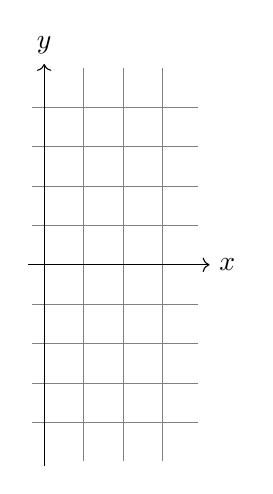
\begin{tikzpicture}[scale=0.5,domain=-0.175782:0.734]
            \draw[very thin,color=gray] (-0.3,-4.99) grid (3.9,4.99);
            \draw[->] (-0.4,0) -- (4.2,0) node[right] {$x$};
            \draw[->] (0,-5.1) -- (0,5.1) node[above] {$y$};
            \draw[color=red] plot function{sqrt(x**6 + 8*x**5 + 22*x**4 + 22*x**3 + 5*x**2 + 6*x + 1)}; 
            \draw[color=red] plot function{-sqrt(x**6 + 8*x**5 + 22*x**4 + 22*x**3 + 5*x**2 + 6*x + 1)}; 
        \end{tikzpicture}
        \end{center}
        {\vspace{-10pt}\caption{Curve, $y^2 = x^6 + 8x^5 + 22x^4 + 22x^3 + 5x^2 + 6x + 1$}}
	    \end{subfigure}%-0.175782
	    ~
	    \begin{subfigure}[t]{0.33\textwidth}
	    \begin{center}
        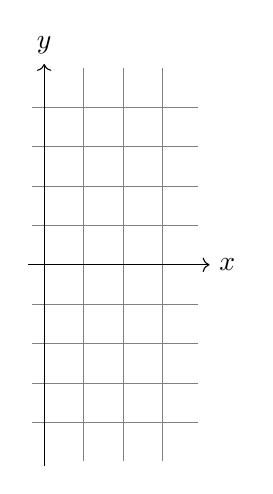
\begin{tikzpicture}[scale=0.5,domain=0:3.63]
            \draw[very thin,color=gray] (-0.3,-4.99) grid (3.9,4.99);
            \draw[->] (-0.4,0) -- (4.2,0) node[right] {$x$};
            \draw[->] (0,-5.1) -- (0,5.1) node[above] {$y$};
            \draw[color=red] plot[samples=200] function{sqrt(x*(x-1)**2)}; 
            \draw[color=red] plot[samples=200] function{-sqrt(x*(x-1)**2)}; 
        \end{tikzpicture}
        \end{center}
        {\vspace{-10pt}\caption{Not a curve, $y^2 = x(x-1)^2$}}
	    \end{subfigure}%
	    ~
	    \begin{subfigure}[t]{0.33\textwidth}
	    \begin{center}
        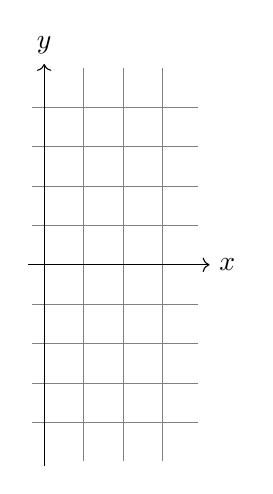
\begin{tikzpicture}[scale=0.5,domain=0:2.6258]
            \draw[very thin,color=gray] (-0.3,-4.99) grid (3.9,4.99);
            \draw[->] (-0.4,0) -- (4.2,0) node[right] {$x$};
            \draw[->] (0,-5.1) -- (0,5.1) node[above] {$y$};
            \draw[color=red] plot function{sqrt(x**3 + x**2)}; 
            \draw[color=red] plot function{-sqrt(x**3 + x**2)}; 
        \end{tikzpicture}
        \end{center}
        {\vspace{-10pt}\caption{Not a curve, $y^2 = x^3 + x^2$}}
	    \end{subfigure}%
    \end{figure}
\end{frame}

\begin{frame}{Algebraic geometry}
    That is the geometric way to think about it: what about the algebraic way?\\\pause
    Take an \textit{equation} in two variables $x,y$. For example $f \coloneqq y- x^2 = 0$.\\\pause
    Look at the solution set $Z(f) = \{(a,b) \in \R^2 \mid f(a,b) = 0\}$\\\pause
    Algebraically, we can think about the polynomial ring $\R[x,y]$.\\\pause
    Then $\Hom(\R[x,y],\R) \cong \R^2$,\pause $ g \mapsto g(x,y), (p \mapsto p(a,b)) \mapsfrom (a,b)$.\\\pause
    Now instead consider $\Hom(\R[x,y]/(y-x^2), \R)$. \\\pause
    Maps to $\R^2$ by $g \mapsto g(x,y)$.\\\pause
    For $g \in \Hom(\R[x,y]/(y-x^2),\R)$ we have that $g(y-x^2) = 0$ so $g(y) - g(x^2) = 0$.\\\pause
    Hence $\Hom(\R[x,y]/(y-x^2), \R) \cong Z(f)$.\\\pause
    \vspace{10pt}
    Correspondence between algebra and geometry!
\end{frame}

\begin{frame}{Algebraic geometry}
    So we have a correspondence: equations correspond to curves, with solutions corresponding to points.\\\pause
    Now we want to look at rational solutions; both $x$ and $y$ should be rational\\\pause
    Or equivalently \textit{rational points}, as they correspond to points on the curve with rational coordinates.\pause
    \begin{center}
    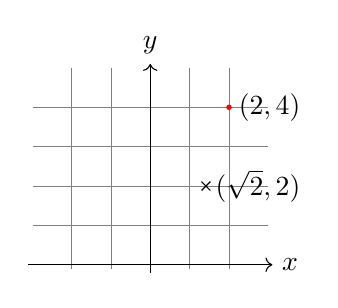
\begin{tikzpicture}[scale=0.5,domain=-2.236:2.236]
            \draw[very thin,color=gray] (-2.99,-0.1) grid (2.99,4.99);
            \draw[->] (-3.1,0) -- (3.1,0) node[right] {$x$};
            \draw[->] (0,-0.2) -- (0,5.1) node[above] {$y$};
            \draw (2,4) node[right] {$(2,4)$};
            \fill[red] (2,4) circle (2pt);
            \draw (1.4142,2) node[right] {$(\sqrt{2},2)$};
            \draw (1.4142,2) node[cross=2pt] {};
            \draw[color=red] plot[samples=200] function{x**2}; 
            %\draw[color=red] plot[samples=200] function{-sqrt(x*(x-1)**2)}; 
    \end{tikzpicture}
    \end{center}
\end{frame}

\begin{frame}{Rational points}
    The parabola $y-x^2 = 0$ has infinitely many rational points!\\ \pause
    When $x$ is rational, so is $x^2$, and there are infinitely many rationals.\\ \pause
    It turns out that this is atypical behavior, occurring because the equation is so simple.~\pause
    Most curves have only finitely many rational points (proven by Faltings in 1983). We take such a curve {\color{red}$C$}\\
    \vspace{-10pt}\begin{figure}
		\centering
		\begin{subfigure}[t]{0.5\textwidth}
		\begin{center}
        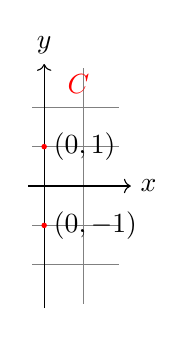
\begin{tikzpicture}[scale=0.5,domain=-0.175782:0.483942]
            \draw[very thin,color=gray] (-0.3,-2.99) grid (1.9,2.99);
            \draw[->] (-0.4,0) -- (2.2,0) node[right] {$x$};
            \draw[->] (0,-3.1) -- (0,3.1) node[above] {$y$};
            \draw[color=red] plot function{sqrt(x**6 + 8*x**5 + 22*x**4 + 22*x**3 + 5*x**2 + 6*x + 1)}; 
            \draw[color=red] plot function{-sqrt(x**6 + 8*x**5 + 22*x**4 + 22*x**3 + 5*x**2 + 6*x + 1)}; 
            \draw (0,1) node[right] {$(0,1)$};
            \fill[red] (0,1) circle (2pt);
            \draw (0,-1) node[right] {$(0,-1)$};
            \fill[red] (0,-1) circle (2pt);
            \draw (0.35,2.6) node[right] {\color{red} $C$};
        \end{tikzpicture}
        \end{center}
	    \end{subfigure}%-0.175782
	    ~
	    \begin{subfigure}[t]{0.5\textwidth}
	    \begin{center}
        \vspace{-70pt}given by \\$y^2 = x^6 + 8x^5 + 22x^4 + 22x^3 + 5x^2 + 6x + 1$.
        \end{center}
	    \end{subfigure}%
    \end{figure}
\end{frame}

\begin{frame}{Solution}
    Recall: we want to find all rational points.\\\pause
    Problem: this set doesn't have a nice structure.\\\pause
    Solution: use sets with a nicer structure.\\
\end{frame}



\begin{frame}{Surfaces}
    Our curve was in the plane, and the plane has a lot of rational points, everywhere!\\\pause
    We embed our curve {\color{red}$C$} in a different, curved surface inside some 15-dimensional space:\\\pause
    \begin{center}
        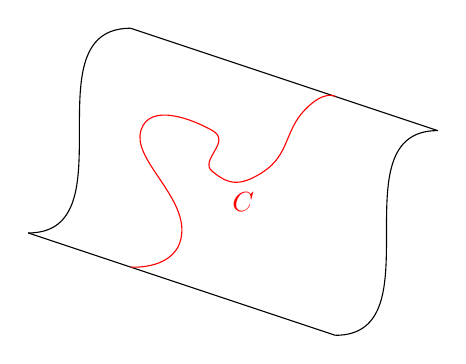
\begin{tikzpicture}[scale=1.3]
            \draw (0,0) .. controls (1,0) and (0,2) ..  (1,2);
            \draw (0,0) -- (3,-1);
            \draw (1,2) -- (4,1);
            \draw (3,-1) .. controls (4,-1) and (3,1) ..  (4,1);
            \draw [red] plot [smooth, tension=1] coordinates { (1,-0.333333) (1.5,0) (1.1,1) (1.8,1) (1.8,0.6) (2.3,0.6) (2.7,1.2) (3,1.3333)};
            \draw (2.1,0.3) node {\color{red} $C$};
        \end{tikzpicture}
    \end{center}
\end{frame}

\begin{frame}{Surfaces}
	This surface has a group structure; we can add any two points on it, and get a third. The rational points form a subgroup isomorphic to $\Z$.\pause~Then the closure of this lies inside a one-dimensional line {\color{blue} $L$}!\pause
	\begin{center}
        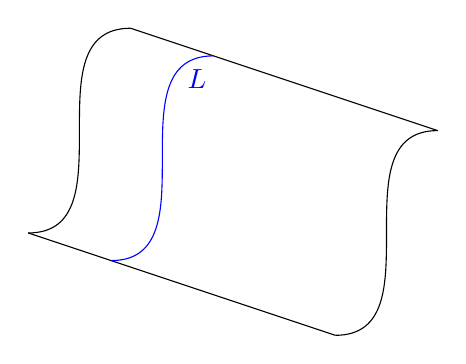
\begin{tikzpicture}[scale=1.3]
            \draw (0,0) .. controls (1,0) and (0,2) ..  (1,2);
            \draw (0,0) -- (3,-1);
            \draw (1,2) -- (4,1);
            \draw (3,-1) .. controls (4,-1) and (3,1) ..  (4,1);
            \draw [blue] (0.81,-0.27) .. controls (1.81,-0.27) and (0.81,1.73) ..  (1.81,1.73);
            \draw (1.65,1.5) node {\color{blue} $L$};
        \end{tikzpicture}
    \end{center}
\end{frame}

\begin{frame}{Final result}
	Now, to find the rational points on the curve we intersect the line {\color{blue} $L$} with the curve {\color{red}$C$} inside this curved surface: \pause
	\begin{center}
        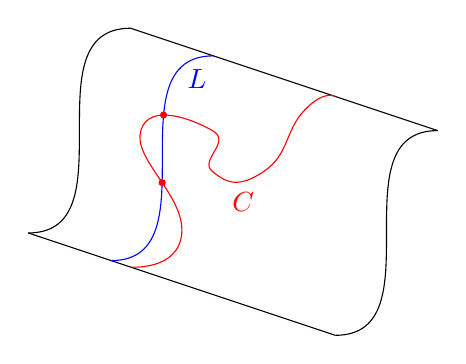
\begin{tikzpicture}[scale=1.3]
            \draw (0,0) .. controls (1,0) and (0,2) ..  (1,2);
            \draw (0,0) -- (3,-1);
            \draw (1,2) -- (4,1);
            \draw (3,-1) .. controls (4,-1) and (3,1) ..  (4,1);
            \draw [name path=C, red] plot [smooth, tension=1] coordinates { (1,-0.333333) (1.5,0) (1.1,1) (1.8,1) (1.8,0.6) (2.3,0.6) (2.7,1.2) (3,1.3333)};
            \draw [name path=L, blue] (0.81,-0.27) .. controls (1.81,-0.27) and (0.81,1.73) ..  (1.81,1.73);
            \draw (1.65,1.5) node {\color{blue} $L$};
            \draw (2.1,0.3) node {\color{red} $C$};
            \fill[red,name intersections={of=C and L}]
    			(intersection-1) circle (1pt)
    			(intersection-2) circle (1pt);
        \end{tikzpicture}
    \end{center}\pause
    Some precision issue's later...\\\pause
    We get there are exactly $2$ points!
\end{frame}

\iffalse
\begin{frame}{Number fields}
	\begin{block}{Question}
		Can we generalise the results of the thesis over a number field $K$?
	\end{block}\pause
	\begin{block}{Answer}
		Yes, in $3$ different ways.
	\end{block}\pause
	\begin{itemize}[<+->]
		\item Embedding $K$ into $\Q_p$ for some $p$, the methods still works the same way if $r \leq g-1$.
		\item Embedding $K$ into $L$ with $L/\Q_p$ of residue field degree $f$, everything should still be fine; this should work if $r \leq f(g-1)$. (If there is an inert prime: if $r \leq d(g-1)$). Maybe: when looking at the $p$-adic completion of the maximal order this works if $r \leq d(g-1)$ if there is no ramification.
		\item Weil restrictions
	\end{itemize}
\end{frame}

\begin{frame}{Weil restriction}
	Let $K$ be a number field of degree $d$, $C_K$ a curve, $J_K$ its Jacobian. Let $X_\Q = \Res_{K/\Q} C_K$ and $A_\Q = \Res_{K/\Q}$, of dimensions $d$ and $dg$ respectively.~\pause
	Consider
	\[
\begin{tikzcd}[ampersand replacement=\&]
\& X_\Q(\Q) \arrow[d] \arrow[r] \& \overline{A_\Q(\Q)} \arrow[d] \arrow[r, no head] \& \dim r\\
\dim d \arrow[r, no head] \& X_\Q(\Q_p) \arrow[r] \& A_\Q(\Q_p)  \arrow[r, no head]  \& \dim dg   
\end{tikzcd}
\]\pause
	We expect this to work if $r \leq d(g-1)$.

\end{frame}
\fi
\end{document}

and (1.5,3) and (2,2)
